%\subsection{Perturbation}
\subsection{Differential Privacy}\label{sec:dp}

Differential Privacy ist eine Technik, welche 2006 von Cynthia Dwork \cite{P-26} vorgestellt wurde.
Ziel dabei ist es, Zugriff auf eine Datenmenge zu ermöglichen, welche sowohl nützliche Erkenntnisse zulässt, als auch die Privatsphäre eines einzelnen Datensatzes schützt.

Differential Privacy kann dabei an 3 unterschiedlichen Stellen der Machine Learning Pipeline genutzt werden:
\begin{compactitem}
\item \textbf{Verfremdung der Trainingsdaten:} Diese Methodik wird folgend in diesem Kapitel erläutert.
\item \textbf{Trainingsalgorithmus:} Kapitel \ref{sec:dp_training} beschreibt, welche Anpassungen am Trainingsalgorithmus vorgenommen werden können, um Differential Privacy zu gewährleisten.
\item \textbf{Vorhersage des Modells:} Bevor die Vorhersage des Modells weitergeleitet wird, könnte diese verrauscht werden. Kapitel \ref{sec:betrieb} stellt dieses Vorgehen vor.
\end{compactitem}

Differential Privacy \cite{P-26} sorgt dafür, dass ein Mechanismus, auch Abfrage oder Funktion, welche eine Menge an Datensätzen als Eingabe akzeptiert, keinen konstanten Wert mehr zurückgibt.
Stattdessen wird dem Mechanismus zufälliges Rauschen mit einer festgelegten Intensität hinzugefügt.
Der Mechanismus gibt also eine Stichprobe einer Verteilung zurück, bei der das tatsächliche Ergebnis dem Erwartungswert entspricht.
Demnach können eindeutige Feststellungen über Eigenschaften nicht getroffen werden.
Ziel des Verrauschens ist es, dass wenn der Mechanismus auf zwei Datenmengen, die sich in einem Datensatz unterscheiden, ausgeführt wird, die Ergebnisse sich maximal um einen Faktor $e^\epsilon$ unterscheiden. 
Demnach ist der Einfluss eines Datensatzes auf eine Berechnung mit der gesamten Datenmenge quantifizierbar und kann begrenzt werden.
Dabei kann der Wert $\epsilon$, welcher auch Privacy Budget genannt wird, festgelegt werden.

Formal lautet die Definition von $\epsilon$-Differential Privacy wie folgt \cite{P-26}:\\
\textit{
Ein randomisierter Mechanismus $M$, welche eine Menge an Datensätzen $D$ auf einen Wertebereich $R$ abbildet, weist $\epsilon$-Differential Privacy auf, wenn für alle Mengen an Datensätze $D_{1}$ und $D_{2}$ die sich in höchstens einem Datensatz unterscheiden $||D_{1} - D_{2}||_{1} \leq 1$ , gilt:}
\begin{equation}
\resizebox{!}{0.3cm}{$
    P[M(D_{1}) \in R] \leq e^{\epsilon} \times P[M(D_{2}) \in R]
$}
\end{equation}
\textit{$P$ beschreibt dabei die Wahrscheinlichkeit, dass der Erwartungswert gezogen wird.}

Es gibt unterschiedliche Algorithmen, um das Ergebnis eines Mechanismus zu verrauschen.
Diese werden im späteren Verlauf des Kapitels genauer beleuchtet.

Dwork und Roth \cite{P-27} fügten der Definition noch einen Parameter $\delta$ hinzu, welcher erlaubt, dass die Bedingungen von $\epsilon$-Differential Privacy zu einem definierten Grad verletzt werden können.
Der Wert von $\delta$ sollte dabei niedriger sein, als die Inverse der Anzahl an Datensätzen im Datenbestand.
Die damit angepasste Definition von ($\epsilon$,$\delta$)-Differential Privacy lautet \cite{P-27}:\\
%Damit lautet die formale Definition von Differential Privacy wie folgt \cite{P-27}:
\textit{
Ein randomisierter Mechanismus $M$, welche eine Menge an Datensätzen $D$ auf einen Wertebereich $R$ abbildet, erfüllt ($\epsilon$,$\delta$)-Differential Privacy, wenn für alle Mengen an Datensätze $D_{1}$ und $D_{2}$ die sich in höchstens einem Datensatz unterscheiden $||D_{1} - D_{2}||_{1} \leq 1$ , gilt:}
\begin{equation}
\resizebox{!}{0.3cm}{$
    P[M(D_{1}) \in R] \leq e^{\epsilon} \times P[M(D_{2}) \in R] + \delta
$}
\end{equation} 

Konkret sagen die Definitionen aus, dass eine randomisierte Funktion $M$, auf zwei Datenbeständen $D_{1}$ und $D_{2}$ mit maximal einem unterschiedlichen Datensatz $||D_{1} - D_{2}||_{1} \leq 1$, jeweils Stichproben einer Verteilung ausgibt, wobei sich die Verteilungen nur um den Faktor $\epsilon$ und den Summand $\delta$ unterscheiden dürfen.
Dabei bestimmt das Privacy Budget, $\epsilon$ und $\delta$, wie stark sich die Ergebnisse unterscheiden dürfen.
Wie diese beiden Werte konfiguriert werden können, hängt dabei vom Algorithmus des Rauschens ab.

\subsubsection*{Konfiguration des Privacy Budgets}

Der $\delta$-Wert wird oftmals als konstanter Wert festgelegt, wobei dieser kleiner als die Inverse der Anzahl an Datensätzen im Datenbestand sein sollte \cite{P-27}.
Die Wahl von $\epsilon$ ist daher entscheidend. 
Abbildung \ref{fig:dp_privacy_budget} zeigt den Einfluss des $\epsilon$-Werts auf die Nützlichkeit und die Vertraulichkeit von Mechanismen.
Kleine Werte für $\epsilon$, also ein kleines Privacy Budget, bedeutet dabei, dass die Differenz eines Mechanismus durch einen zusätzlichen Datensatz, sich weniger stark verändern kann, was für einen besseren Schutz der Privatsphäre sorgt.
Jedoch wirkt sich dies negativ auf die Nützlichkeit der Abfragen aus, da kleine Privacy Budgets für ein großes Rauschen sorgen, was öfters falsche Ergebnisse liefert.
Dies bedeutet, dass es keinen optimalen Wert für $\epsilon$ gibt, sondern dieser für jeden Use Case mittels einer Abwägung zwischen Sicherheit und Nützlichkeit, neu bestimmt werden muss.
Nutzt ein Modell beispielsweise nur öffentliche, unsensible Daten, ergibt es keinen Sinn einen niedrigen $\epsilon$-Wert festzulegen, da die Vertraulichkeit der Daten nicht entscheidend ist.
Werden jedoch hochsensible Daten genutzt, kann es sein, dass die Sicherheit der Daten wichtiger eingestuft wird, als die Nützlichkeit des Modells. 
Hier empfiehlt sich ein niedriger $\epsilon$-Wert.
Ein $\epsilon$-Wert von Unendlich bedeutet, dass sich die Ergebnisse von Mechanismen um beliebige Werte unterscheiden dürfen, weshalb kein Rauschen notwendig wäre. 
Dies ist bei Mechanismen ohne Differential Privacy bereits der Fall.

\begin{figure}[!htb]
    \centering
    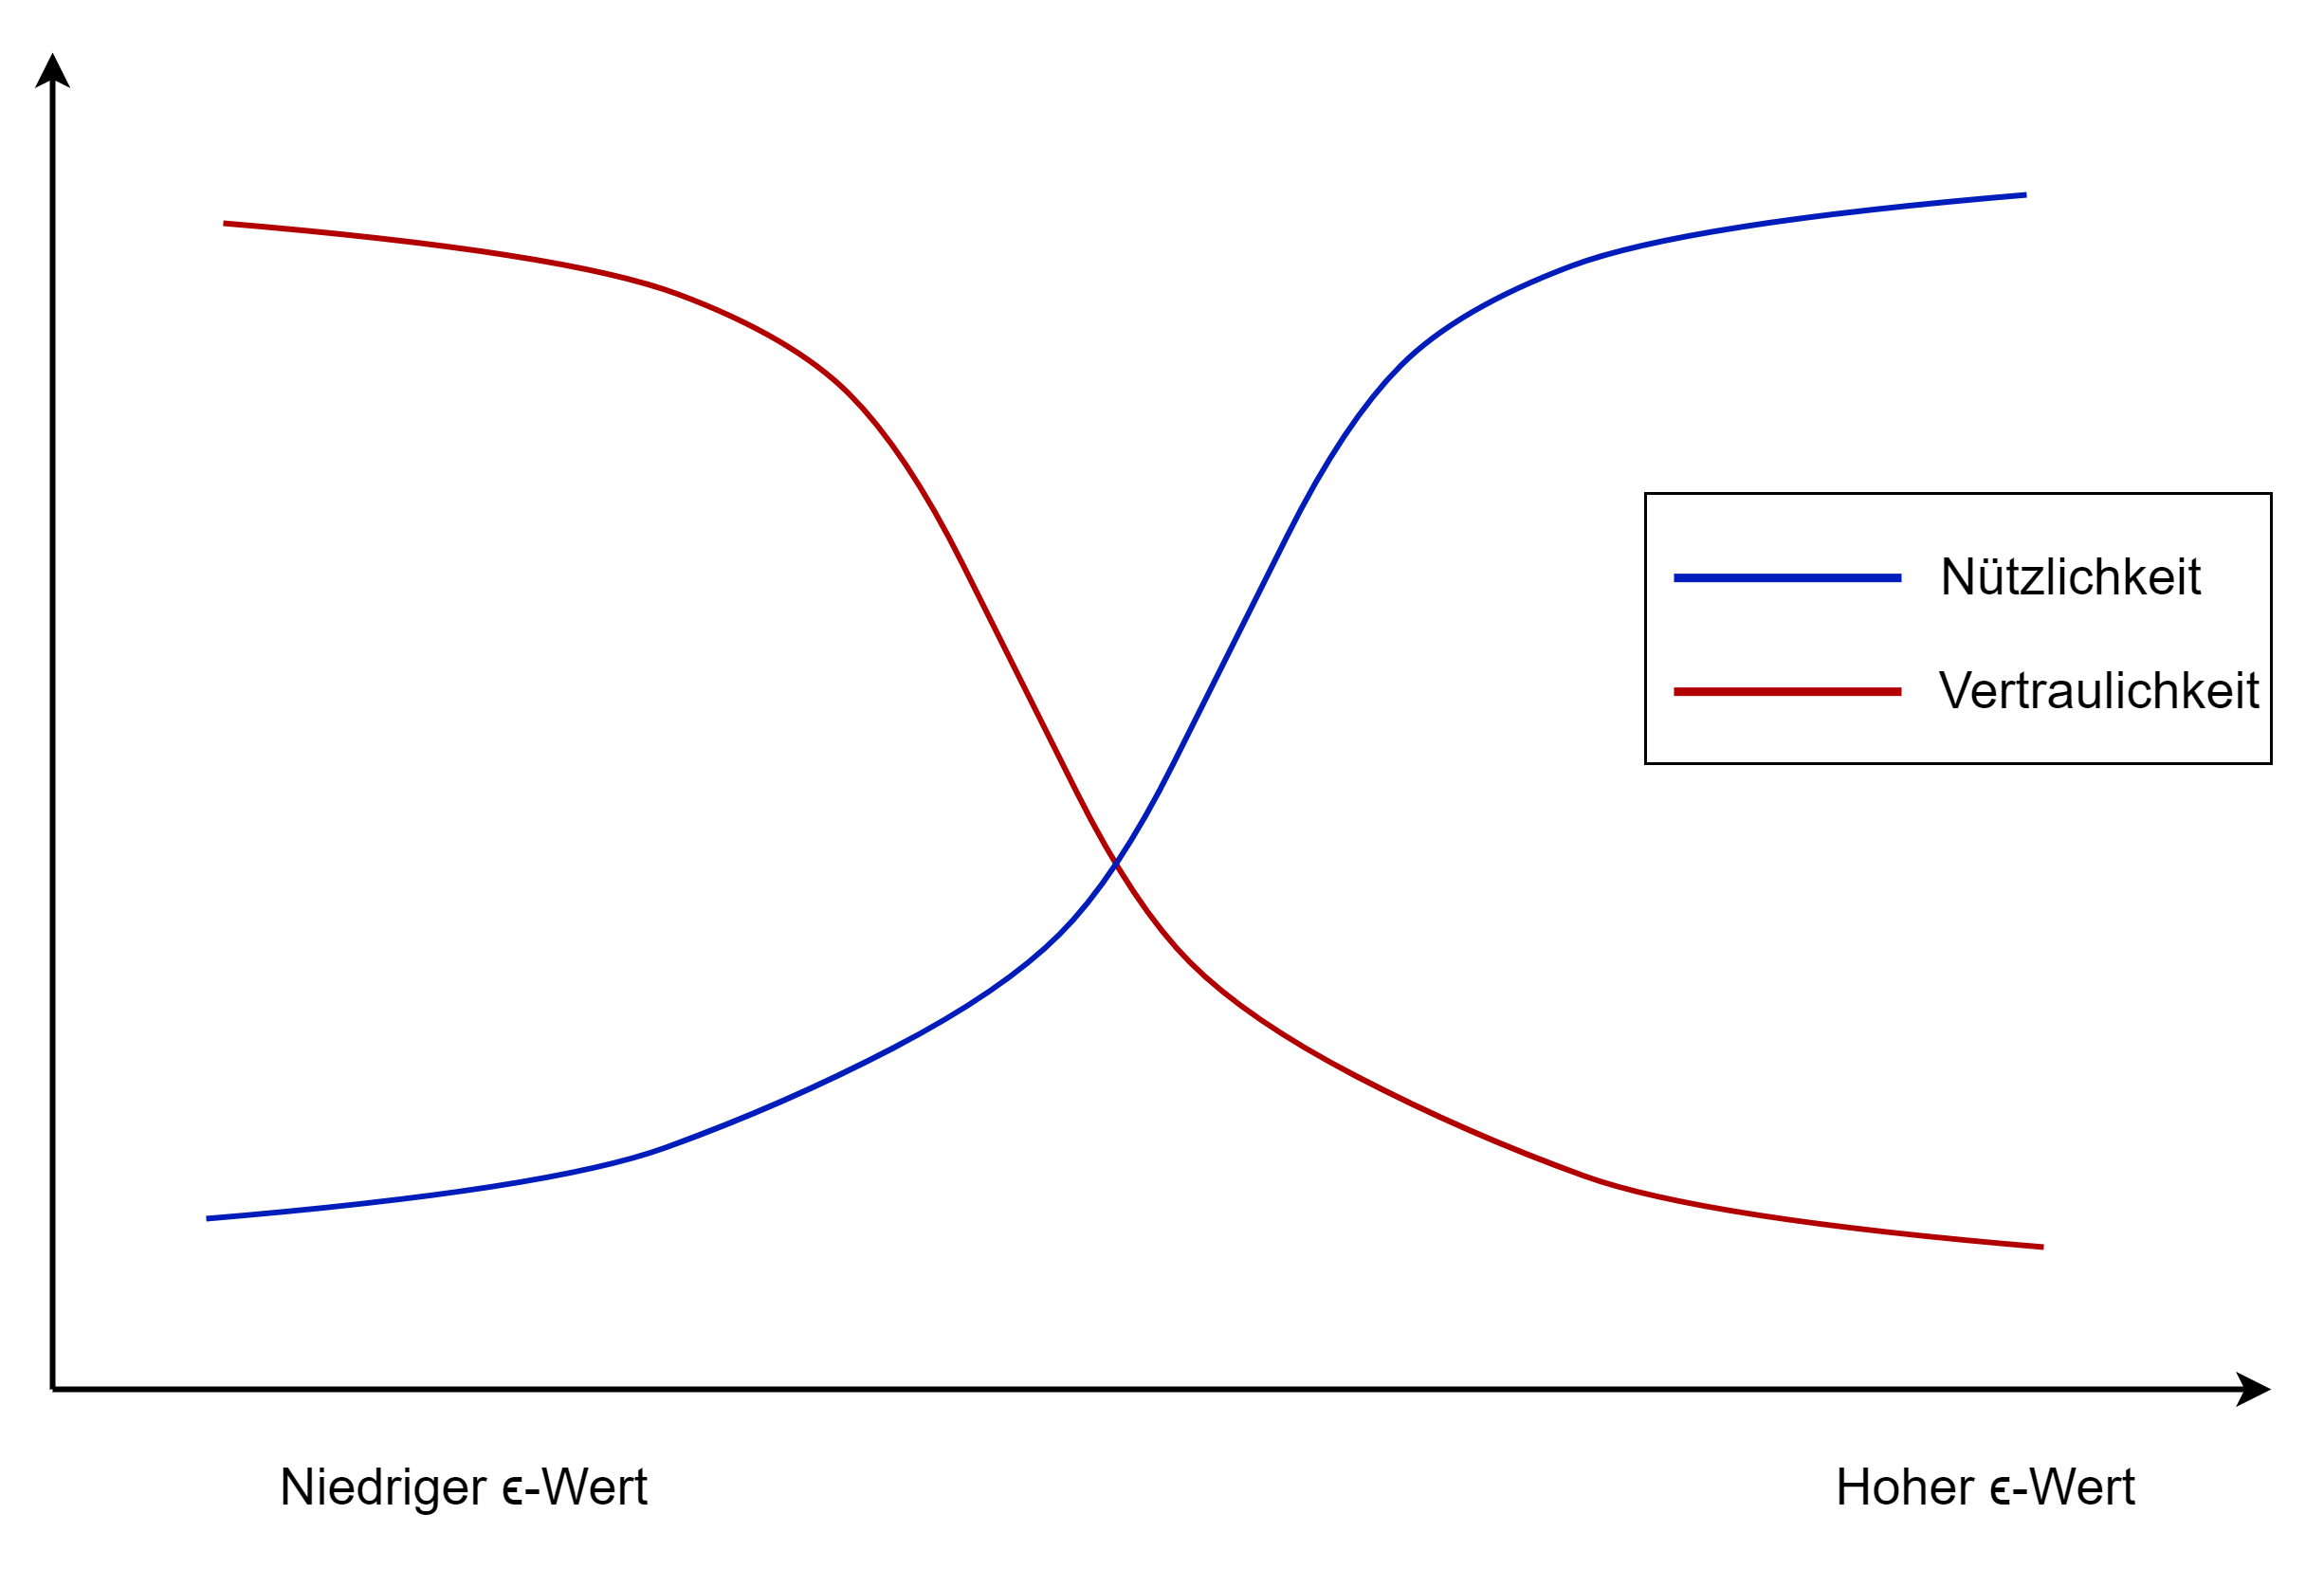
\includegraphics[width=12cm]{figures/dp_privacy_budget.png}
    \caption{Einfluss von $\epsilon$}
    \label{fig:dp_privacy_budget}
\end{figure} 

\subsubsection*{Beispiel für Differential Privacy}

Abbildung \ref{fig:dp} zeigt, wie sich Abfragen mit und ohne Differential Privacy unterscheiden.
Dabei führt ein Angreifer zunächst eine Abfrage über das Durchschnittsgehalt eines Unternehmens auf einem Datenbestand ohne Differential Privacy aus. 
Er erhält hier einen konkreten Wert als Ergebnis.
Anschließend wird der Datenbestand um einen Eintrag erweitert, weil das Unternehmen einen neuen Mitarbeiter hat.
Führt der Angreifer die Abfrage um das Durchschnittsgehalt erneut aus, erhält dieser einen angepassten, neuen Wert.
Dadurch kann er anhand der Anzahl der Mitarbeiter des Unternehmens und der Differenz der beiden Abfragen das exakte Gehalt des neuen Mitarbeiters bestimmen.
Anders sieht dies mit Differential Privacy aus. 
Dabei werden beide Abfragen mit zufälligem Rauschen angereichert. 
Es wird also nur eine Stichprobe einer Verteilung zurückgegeben. 
Bei einer gleichen Abfrage auf den gleichen Datenbestand, können also ebenfalls unterschiedliche Werte zurückgegeben werden.
Führt der Angreifer zwei Abfragen aus, einmal auf dem alten Datenbestand und auf dem Datenbestand mit dem neuen Mitarbeiter, kann er keinen exakten Wert des Gehalts des neuen Mitarbeiters ermitteln.
Differential Privacy bietet einige Algorithmen, wie dieses Rauschen hinzugefügt werden kann, wobei Parameter $\epsilon$ und $\delta$ die Stärke des Rauschens bestimmen und damit auch, wie nah die beiden Ergebnisse aneinander sind.

\begin{figure}[!htb]
    \centering
    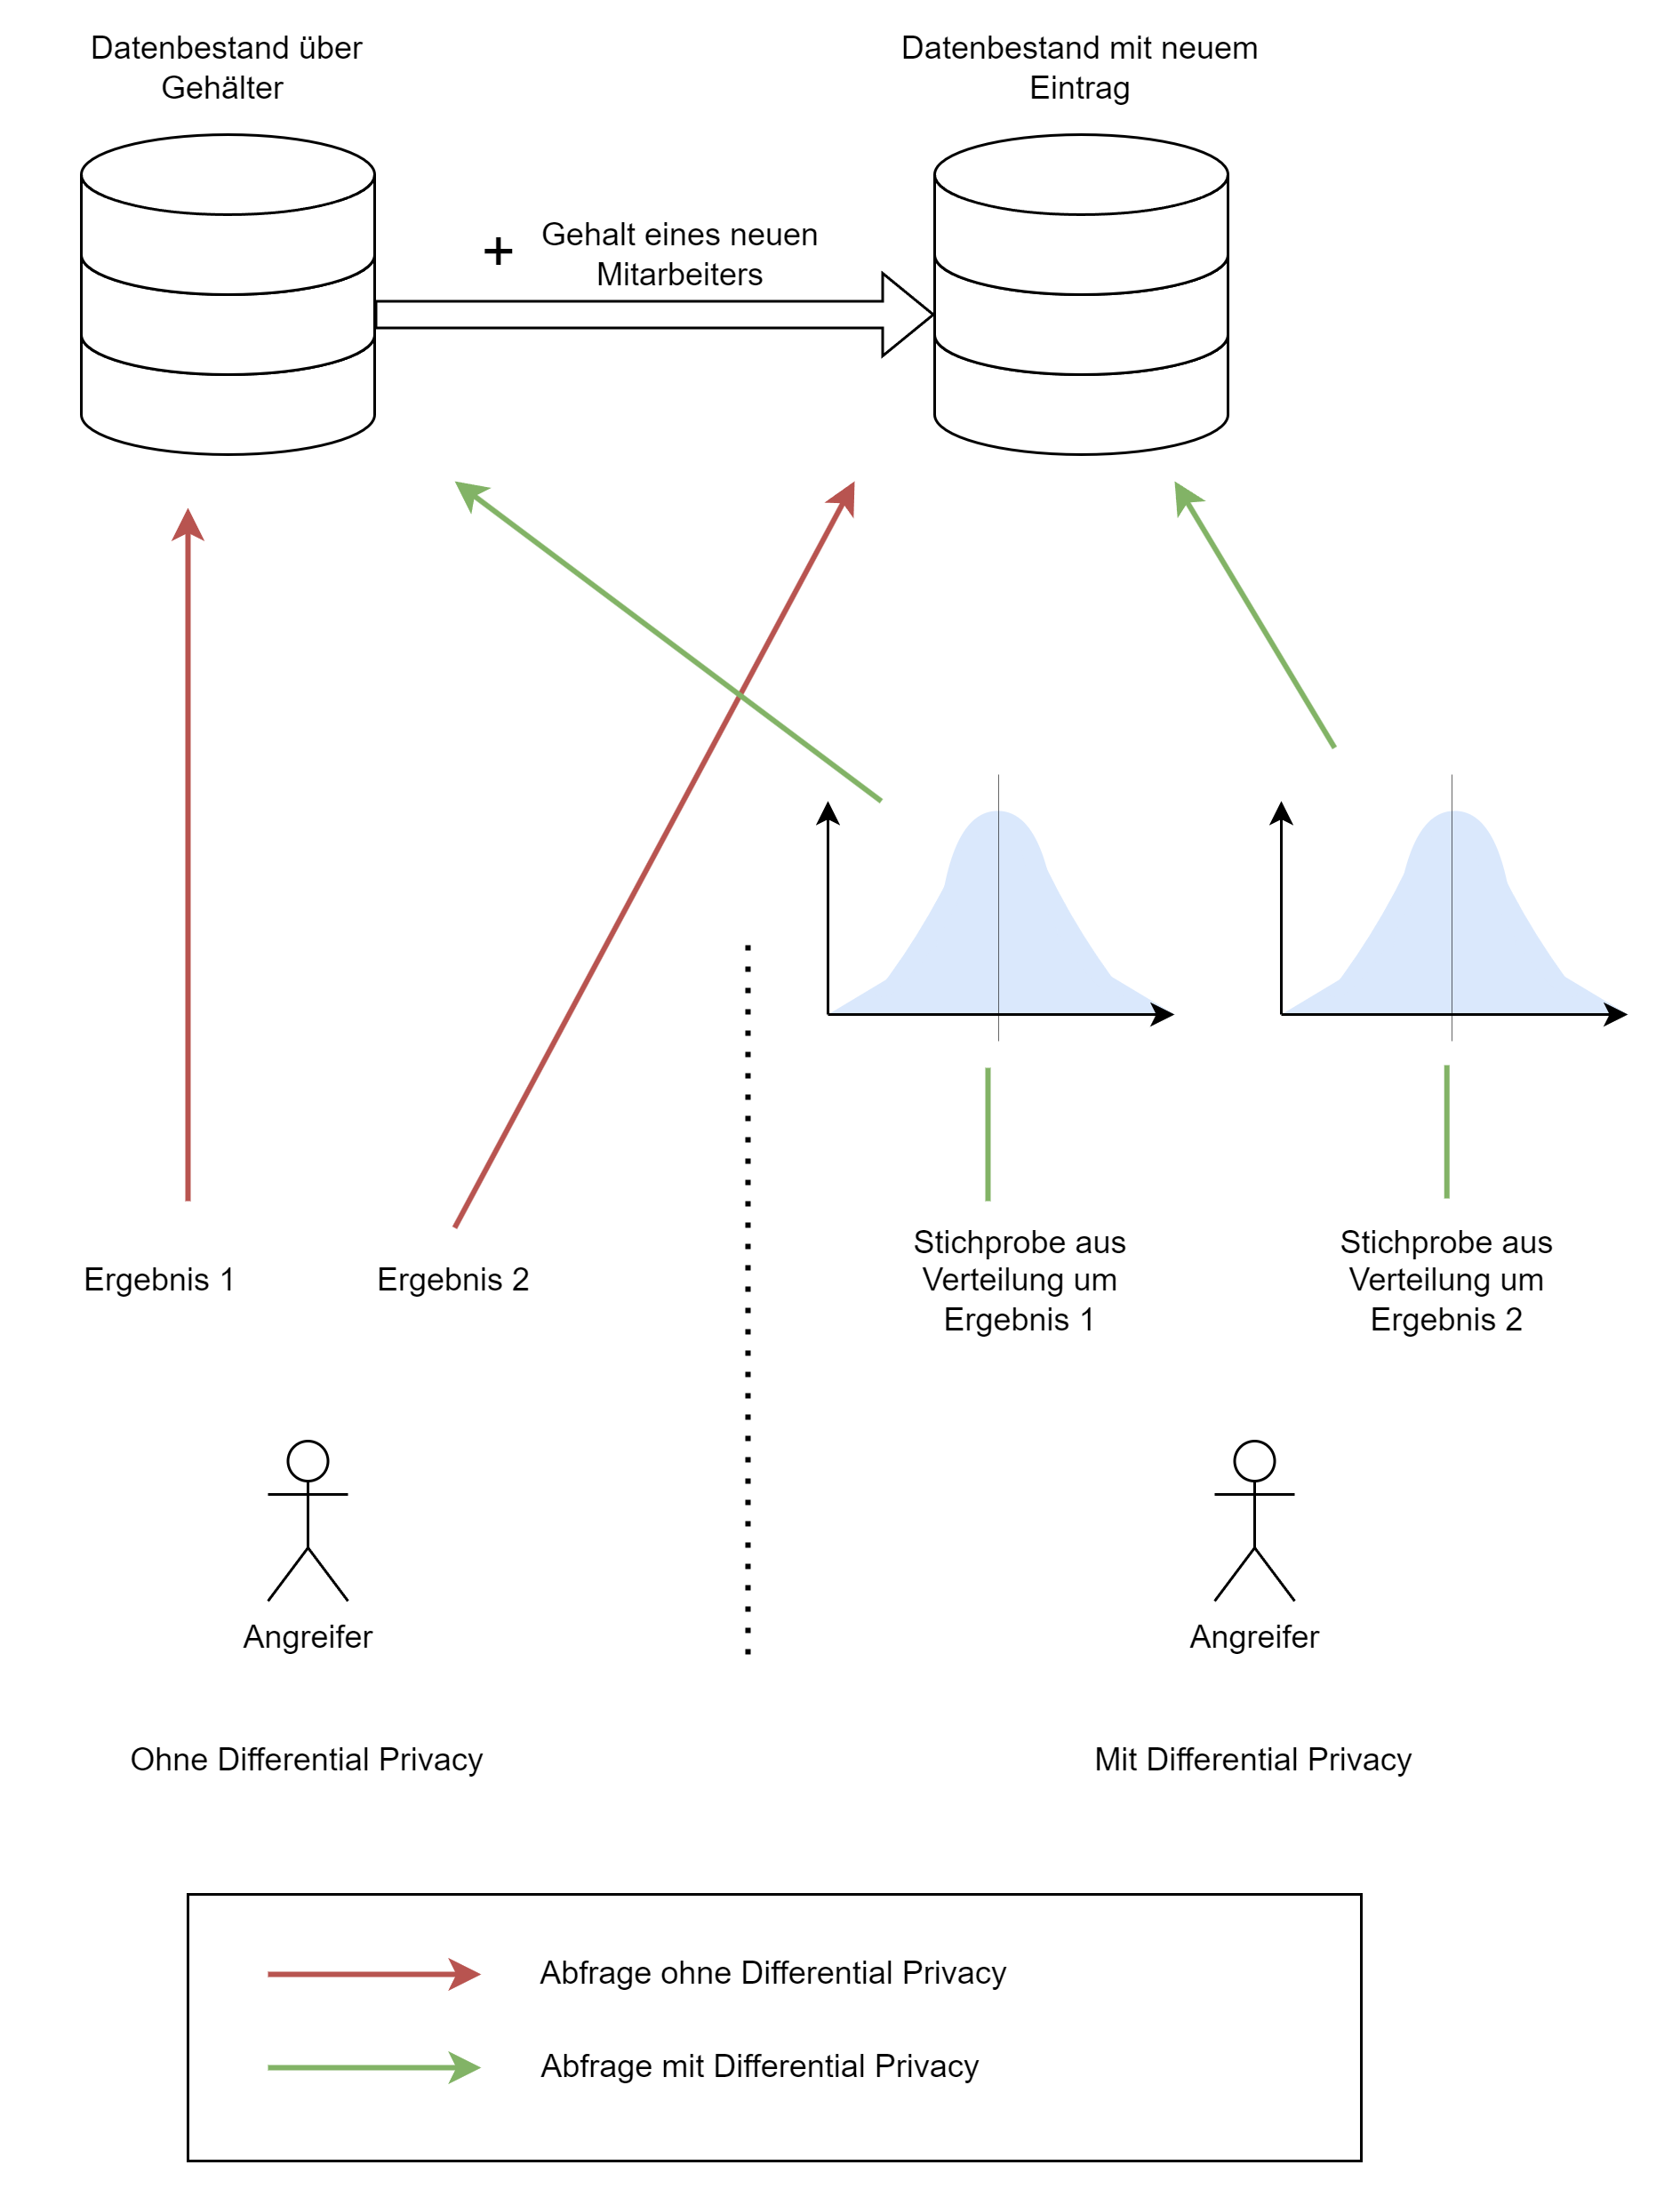
\includegraphics[width=\textwidth]{figures/dp}
    \caption{Beispiel Differential Privacy}
    \label{fig:dp}
\end{figure} 

\subsubsection*{Algorithmen für Differential Privacy}
Die Art des Rauschens, welche über die Ausgabe einer Abfrage gelegt wird, kann unterschiedlichster Herkunft sein.
Dwork und Roth \cite{P-27} stellen eine ganze Reihe dieser Mechanismen vor, die im Folgenden beschrieben werden.

Bei der Technik der randomisierten Antwort, im Englischen Random Response, wird mit einer festgelegten Wahrscheinlichkeit, ein falsches Ergebnis ausgegeben. 
Dies entspricht dem Rauschen dieser Methode.
Wird beispielsweise eine Person gefragt, ob sie eine gewisse Aktivität durchgeführt hat, wird mit 25-prozentiger Wahrscheinlichkeit die falsche Antwort selektiert.
Ist die Wahrheit \textit{\dq Ja\dq}, dann gilt $P[Antwort = \dq Ja\dq \mid Wahrheit = \dq Ja\dq] = 3/4$ und $P[Antwort = \dq Nein\dq \mid Wahrheit = \dq Ja\dq]$.
Gleiches gilt, wenn die Wahrheit \textit{\dq Nein\dq} wäre.
Die jeweils ausgegebene Antwort kann dadurch glaubhaft abgestritten werden.
\begin{equation} \label{formula:random_response}
\begin{split}
\frac{P[Antwort = \dq Ja\dq \mid Wahrheit = \dq Ja\dq]}{P[Antwort = \dq Ja\dq \mid Wahrheit = \dq Nein\dq]} = \frac{3/4}{1/4} = \\
\frac{P[Antwort = \dq Nein\dq \mid Wahrheit = \dq Nein\dq]}{P[Antwort = \dq Nein\dq \mid Wahrheit = \dq Ja\dq]} =  3
\end{split}
\end{equation}

Formel \ref{formula:random_response} zeigt, dass eine Antwort, egal ob diese \textit{\dq Ja\dq} oder \textit{\dq Nein\dq} lautet, mit einem Verhältnis von 3 abgestritten werden kann.
Der Faktor, um den sich die Wahrscheinlichkeit einer Antwort unterscheidet, wenn sich die Wahrheit ändert, liegt demnach auch bei 3.
Daraus resultiert, dass die Technik der randomisierten Antwort, mit einer 25-prozentigen Wahrscheinlichkeit einer falschen Antwort, eine ($ln 3$, 0)-Differential Privacy unterstützt.
Der natürliche Logarithmus $ln$ muss hier genutzt werden, da die Definition von Differential Privacy die Exponentialfunktion als Faktor betrachtet. 
Demnach erhält man durch $\epsilon = ln 3$ einen Unterschied um den Faktor $e^{ln 3} = 3$.

Eine weitere Technik für Differential Privacy ist der Laplace-Mechanismus.
Dabei wird das Rauschen, welches über das Ergebnis der Abfrage gelegt wird, aus einer Laplace-Verteilung ermittelt.
Eine Bedingung ist dabei, dass es sich bei dem Ergebnis der Abfrage um einen Zahlenwert handelt.
Die Dichtefunktion der Laplace-Verteilung, zentriert um den Erwartungswert $\mu=0$, mit dem Skalenparameter $\sigma$, lautet \cite{P-27}:
\begin{equation}
\resizebox{!}{0.55cm}{$
    Lap(x|\sigma) = \frac{1}{2\sigma}\times e^{(-\frac{|x|}{\sigma})}
$}
\end{equation}
wobei $\sigma$ die Steigung der Funktion beeinflusst.
Um nun ein geeignetes $\sigma$ zu wählen, muss zuerst ein Wert ermittelt werden, um den sich eine Funktion bei Änderung eines Datenpunktes maximal unterscheiden kann.
Diese sogenannte Sensitivität wird als $\Delta f$ notiert.
Geht es beispielsweise um eine Anzahl an Datensätzen, so würde ein neuer Datensatz die Anzahl um den Wert 1 erhöhen.
Folglich ist $\Delta f = 1$, denn die Anzahl wird sich durch einen neuen Datensatz um den Wert 1 verändern.
Es gibt jedoch auch Fälle, in denen der Wert der Sensitivität nicht eindeutig ist, beispielsweise bei dem obigen Gehaltsbeispiel.
Das Gehalt einer neuen Person könnte für eine beliebige Veränderung des Durchschnittsgehalts sorgen, da theoretisch jedes Gehalt möglich wäre.
Realistisch betrachtet gibt es jedoch einen Wertebereich, in dem sich alle Gehälter befinden. 
Dieser könnte beispielsweise von 0 Euro bis 10 Milliarden Euro reichen. 
Jedoch sollten die Grenzen möglichst nahe an den echten Grenzen liegen. 
10 Milliarden Euro ist theoretisch möglich, jedoch ist eine Grenze von 200.000 Euro realistischer.
Dieser Wertebereich muss also fachlich festgelegt werden.
In diesem Beispiel wäre die Sensitivität $200.000/n$, wobei $n$ die Anzahl der Mitarbeiter ist.


Um ($\epsilon$,0)-Differential Privacy zu erreichen, muss die Ausgabe einer Abfrage $M$ mit zufälligen Werte der Laplace-Verteilung $Lap(x | \Delta f/\epsilon)$ verrauscht werden \cite{P-27}: 
\begin{equation}
    M(D) = f(D) + (Y_1, ... Y_k),\text{ mit } Y_i \sim Lap(x| \Delta f/\epsilon)
\end{equation}


Eine Abwandlung des Laplace-Mechanismus ist es, anstatt der Laplace-Verteilung, eine Gaußverteilung zu nutzen. Die Dichtefunktion dieser zentriert um den Erwartungswert $\mu=0$ lautet \cite{P-27}:
\begin{equation}\label{formula:gauß}
\resizebox{!}{0.55cm}{$
    Gau\text{\textit{ß}}(x|\sigma) = \frac{1}{\sigma\sqrt{2\pi}}\times e^{-\frac{1}{2}(\frac{x}{\sigma})^2}
$}
\end{equation}
Der Gauß-Mechanismus liefert ($\epsilon$,$\delta$)-Differential Privacy, wenn $\sigma = \Delta f \frac{\text{ln}(1/\delta)}{\epsilon}$ ist \cite{P-27}.

Neben den bereits beschriebenen Mechanismen gibt es noch den Exponential-Mechanismus. 
Bei diesem wird ein Element aus einer Menge ausgegeben, welches anhand einer Bewertungsfunktion ausgewählt wird.
Die Abfrage an einen Datenbestand liefert also keine Zahl, sondern einen Datensatz oder Attributwert aus diesem.
Der Exponential-Mechanismus benötigt eine Bewertungsfunktion $u:D x R \xrightarrow{} \mathbb{R}$, welche für jede potenzielle Ausgabeoption $R$ aus einer Menge an Datensätzen $D$, einen Nutzwert im Wertebereich $\mathbb{R}$ berechnet.
Als Sensitivität $\Delta f$ entspricht der Sensitivität der Bewertungsfunktion $\Delta f = \Delta u$
Die Anfrage erfüllt dabei ($\epsilon$,0)-Differential Privacy, wenn der Mechanismus $M(D,u,R)$ ein Element $r \in R$ auswählt und ausgibt, mit einer Wahrscheinlichkeit proportional abhängig von
\begin{equation}\label{formula:exp_mech}
\resizebox{!}{0.8cm}{$
    e^{\frac{\epsilon \times u(D,r)}{2\Delta u}}
$}
\end{equation}


Als Beispiel könnte ein Mechanismus genutzt werden, welcher ausgeben soll, ob Krankheit \dq A\dq\ oder \dq B\dq\ häufiger vorkommt.
Somit wären die möglichen Optionen $R$=\{\dq A\dq,\dq B\dq\}, die Bewertungsfunktion $u(D,r)=\text{Count(r in D)}$.
Die Sensitivität ist $\Delta u = 1$, da ein zusätzlicher Datensatz die Zählung maximal um die Anzahl 1 verändern kann. 
Für jede der Optionen in $R$, würde die Ausgabewahrscheinlichkeit mit Formel \ref{formula:exp_mech} berechnet werden. 
Anschließend gibt der Mechanismus entweder \dq A\dq\ oder \dq B\dq\ zurück, abhängig der zuvor berechneten Ausgabewahrscheinlichkeiten.
Das Rauschen des Exponential-Mechanismus ist demnach, dass nicht immer die Option $r \in R$ mit dem größten Nutzwert ausgegeben wird. 

Eine alternative Möglichkeit, neben dem Exponential-Mechanismus, einen Wert aus einem Datensatz mittels Ausgabewahrscheinlichkeiten zu bestimmen, ist die sogenannte Report Noisy Max Methode. 
Dabei werden die echten Wahrscheinlichkeitswerte mittels Laplace-Mechanismus verrauscht und anschließend wird der Wert oder Datenpunkt mit der höchsten Wahrscheinlichkeit selektiert.


\subsubsection*{Eigenschaften von Differential Privacy}
Das Ziel von Differential Privacy, die Vertraulichkeit eines Datensatzes zu schützen und dennoch die Nützlichkeit des Datenbestands zu bewahren, wurde bereits zu Beginn des Kapitels geschildert.
Jedoch bringt Differential Privacy eine Reihe weiterer nützlicher Eigenschaften mit sich \cite{P-27}:
\begin{compactitem}
    \item \textbf{Gruppen Privacy:} Differential Privacy betrachtet zwei Datenbestände, die sich in einem Datensatz unterscheiden. Jedoch gelten die gleichen Regeln für Datenbestände, die sich in mehreren Datensätzen unterscheiden, wobei $\epsilon$ dabei mit der Anzahl der unterschiedlichen Datensätze multipliziert wird.
    \item \textbf{Resistenz gegen Umkehrung bei der Weiterverarbeitung:} Das Ergebnis eines Mechanismus, welcher Differential Privacy nutzt, ist geschützt und es gibt keinen Mechanismus, welcher dies umkehren könnte. Somit sind geschützte Weiterverarbeitungen der Ergebnisse möglich.
    \item \textbf{Quantifizierung der Vertraulichkeit:} Mit den Parametern $\epsilon$ und $\delta$ kann angegeben werden, wie stark die Vertraulichkeit der Daten geschützt wird.
    \item \textbf{Bewertung zusammengesetzter Mechanismen:} Durch die Quantifizierung der Vertraulichkeit, können auch zusammengesetzte und parallele Berechnungen bewertet werden.
\end{compactitem}



Die Bewertung von mehreren zusammengesetzten Mechanismen ist dabei komplex und kann für bestimmte Berechnungen verfeinert werden \cite{P-27}. 
Der dabei berechnete $\epsilon$-Wert ist eine Obergrenze, welcher durch bestimmte Restriktionen und Berechnungen noch genauer definiert werden kann.
Grundlegend jedoch, besitzt ein Mechanismus, welcher aus nacheinander ausgeführten Teilmechanismen besteht, einen $\epsilon$-Wert und $\delta$-Wert, welcher der Summe aus den einzelnen Teilmechanismen entspricht.
Erfüllt $M_1(D)$ eine $(\epsilon_1,\delta_1)$-Differential Privacy und $M_2(D)$ eine $(\epsilon_2,\delta_2)$-Differential Privacy, dann erfüllt der gesamte Mechanismus $(\epsilon_1 + \epsilon_2,\delta_1 + \delta_2)$-Differential Privacy.
Wird ein und derselbe Teilmechanismus mit $(\epsilon,\delta)$-Differential Privacy $t$ mal ausgeführt, so entspricht der Gesamtmechanismus $(t\epsilon,t\delta)$-Differential Privacy.
Zusammengefasst lässt sich dies durch folgende Definition beschreiben \cite{P-27}:\\
\textit{
    Wenn ein Mechanismus $M_{|t|}$, aus $t$ Teilmechanismen $M_i$ mit $(\epsilon_i,\delta_i)$-Differential Privacy besteht, dann erfüllt dieser  ($\Sigma_{i=1}^{t} \epsilon_i $, $\Sigma_{i=1}^{t} \delta_i $)-Differential Privacy
}

Alternativ kann ein Mechanismus auch aus Teilmechanismen bestehen, welche jeweils nur auf einer disjunkten Menge an Datensätzen des gesamten Datenbestands ausgeführt wird.
Der gesamte Mechanismus hat als $\epsilon$ und $\delta$-Wert dabei die maximalen Werte der Teilmechanismen.\\
\textit{
    Wenn ein Mechanismus $M_{|t|}$, aus $t$ Teilmechanismen $M_i$ mit $(\epsilon_i,\delta_i)$-Differential Privacy besteht, welche jeweils 
    nur auf einer disjunkten Menge an Datensätzes des gesamten Datenbestands $D_i$ ausgeführt werden, 
    dann erfüllt dieser Mechanismus ($max_i(\epsilon_{i})$, $max_i(\delta_{i})$)-Differential Privacy
}


Ein Beispiel für einen Algorithmus, welcher eine angepasste Bewertung von zusammengesetzten Mechanismen besitzt, ist der Trainingsalgorithmus DPSGD (Kapitel \ref{sec:dp_training}) \cite{P-28}.
Diese Anpassung sorgt dafür, dass der $\epsilon$-Wert über den ganzen Trainingsprozess möglichst niedrig bleibt.
Ziel davon ist es, eine Obergrenze für $\epsilon$ zu beschreiben, welche näher an den tatsächlichen Berechnungen liegt, als das Aufsummieren der einzelnen $\epsilon$ Werte.


\subsubsection*{Vorverarbeitung der Trainingsdaten}
Um die Trainingsdaten eines Modells mit Differential Privacy zu schützen, ist es möglich, die Daten vor der Eingabe in das Modell zu verrauschen.
Der Forward-Pass eines Modells wird demnach nicht auf den echten Daten ausgeführt, sondern auf den jeweils verrauschten Versionen der einzelnen Datensätze.

Um einen einzelnen Datensatz zu verrauschen, muss jedes Attribut des Datensatzes individuell betrachtet werden. 
Dabei ist die Sensitivität individuell zu setzen, beeinflusst von statistischen Merkmalen des Attributes.
Ebenfalls kann sich der Differential Privacy Mechanismus unterscheiden, abhängig davon, ob es sich um kategoriale oder numerische Werten handelt.
Bei numerischen Werten kann der Laplace-Mechanismus oder Gauß-Mechanismus gewählt werden, bei kategorialen Werten der Exponential-Mechanismus.
Der $\epsilon$-Wert und $\delta$-Wert eines einzelnen Datenpunktes entspricht anschließend der Summe der Werte des einzelnen Verrauschens jeder Variable.

Da jeder Datensatz alleine eine disjunkter Menge des Datenbestands darstellt, gilt, dass der $\epsilon$-Wert und $\delta$-Wert dem Maximum des Rauschens auf die einzelnen Datensätze entspricht.
Wird also jeder Datensatz mit dem gleichen, festgelegten Mechanismus mit ($\epsilon$,$\delta$)-Differential Privacy verrauscht, dann entspricht dies auch den Werten des gesamten Vorverarbeitungsprozess.

Alternativ kann ein ganzer Datenbestand mit Differential Privacy geschützt werden, indem dieser nur dazu genutzt wird, einen synthetischen Datenbestand zu erzeugen.
Dieser kann anschließend wie der originale Datenbestand genutzt werden.
Das folgende Kapitel stellt einige Methoden dazu vor.

